\documentclass[a4paper,12pt]{article}

\usepackage{amsmath,amssymb,multicol,tikz,enumitem}
\usepackage[margin=2cm]{geometry}
%\usetikzlibrary{calc}
\usepackage{amsmath}
\usepackage{amsthm}
\usepackage{thmtools}
\usepackage{hyperref}
\usepackage{enumerate}
\usepackage{xcolor}
\usepackage{fancyvrb}

\pagestyle{empty}

\newcommand\Q{\mathbf{Q}}
\newcommand\R{\mathbf{R}}
\newcommand\Z{\mathbf{Z}}

%\newcommand\answer[1]{}
%\newcommand\ans[1]{}
\newcommand\answer[1]{\\[5pt]{\color{blue}{#1}}\hfill{\color{blue}}\\[-5pt]}
\newcommand\ans[1]{{\color{blue}{#1}}}

\usepackage{array}
\newcolumntype{P}[1]{>{\centering\arraybackslash}p{#1}}

\newcommand\indd{${}$\hspace{20pt}}

\declaretheoremstyle[headfont=\normalfont\bfseries,notefont=\mdseries\bfseries,bodyfont = \normalfont,headpunct={:}]{normalhead}
\declaretheorem[name={Uzdevums}, style=normalhead,numberwithin=section]{problem}

\setcounter{section}{01}

\setlength\parindent{0pt}

\renewcommand{\figurename}{Attēls}

\begin{document}

\begin{center}
\parbox{3.5cm}{\flushleft\bf Racionāli, Iracionāli skaitļi} \hfill {\bf\LARGE Sacensības \#2021.04} \hfill \parbox{3.5cm}{\flushright\bf 2021-04-08} \\[2pt]
{\rm\footnotesize Par šo LU NMS atbalstīto pasākumu\\ atbild {\tt kalvis.apsitis@gmail.com}.}
\end{center}

%\hrule\vspace{2pt}\hrule
\hrule

%%%%%%%%%%%%%%%
%%% 01 %%%%%%%%
%%%%%%%%%%%%%%%
\vspace{10pt}
\begin{problem}
Sauksim naturālu skaitli n par {\em derīgu}, ja attēlā dotās izteiksmes vērtība arī ir naturāls skaitlis: 
\[ \sqrt{n^2 + 85n + 2021} \]
Atrast visu derīgo skaitļu summu.

{\bf Jautājums:} Ierakstīt naturālu skaitli \textendash{} visu derīgo $n$ summu.
\answer{

{\bf Atbilde.} $\mathtt{172}$

Pareizinām izteiksmi zem saknes ar $4$, lai būtu vieglāk (bez dalīšanas ar $2$) atdalīt pilno kvadrātu. 
$\sqrt{n^2 + 85n + 2021}$ ir vesels skaitlis tad un tikai tad, ja $\sqrt{4n^2 + 340n + 8084}$ ir vesels
skaitlis jeb $4n^2 + 340n + 8084$ ir pilns kvadrāts $k^2$. Pārrakstām:

\[ 4n^2 + 340n + 8084 = k^2, \]
\[ (2n+85)^2 - 85^2 + 8084 = k^2, \]
\[ (2n+85)^2 + 859 = k^2, \]
Ievērosim, ka $(2n+85)^2 < k^2$ un arī $2n+85 < k$. Atņemam no lielākā pilnā kvadrāta mazāko un dalām reizinātājos:
\[ k^2 - (2n+85)^2 = 859, \]
\[ (k - (2n+85))(k + (2n+85)) = 859. \]
Tā kā $859$ ir pirmskaitlis, to var izteikt naturālu skaitļu reizinājumā tikai vienā veidā:
\[ \left\{ \begin{array}{l} 
k - (2n + 85) = 1,\\
k + (2n + 85) = 859.\\
\end{array} \right. \]
Reizinātāju $1$ un $859$ secību mainīt nevar, jo $k-(2n+85)$ ir mazāks par $k+(2n+85)$. 

Atņemam vienādojumus vienu no otra:
\[ (2n + 85) = \frac{859 - 1}{2} = 429. \]
Tāpēc $2n = 344$ un $n = 172$. 

Var arī pārbaudīt, ja $n = 172$:
\[ \sqrt{n^2 +85n + 2021} = \sqrt{172^2 + 85 \cdot 172 + 2021} = 215. \]
}
\end{problem}


%%%%%%%%%%%%%%%
%%% 02 %%%%%%%%
%%%%%%%%%%%%%%%
\vspace{10pt}
\begin{problem}
Atrast naturālu skaitli $n$, kuram izpildās vienādība:
\[ \lfloor \log_2 1 \rfloor + \lfloor \log_2 2 \rfloor + \lfloor \log_2 3 \rfloor + \ldots + \lfloor \log_2 n \rfloor = 1898. \]
(Formulā ar $\lfloor x \rfloor$ apzīmēta skaitļa $x$ veselā daļa.)

{\bf Jautājums:} Ierakstīt naturālu skaitli $n$, kas apmierina vienādojumu.
\answer{

{\bf Atbilde.} $\mathtt{300}$\\

Aprēķinām dažu pirmo naturālo skaitļu logaritmu veselās daļas:

\[ \begin{array}{l}
\lfloor \log_2 1 \rfloor = 0,\\
\lfloor \log_2 2 \rfloor = \lfloor \log_2 3 \rfloor = 1,\\
\lfloor \log_2 4 \rfloor = \ldots \lfloor \log_2 7 \rfloor = 2,\\
\lfloor \log_2 8 \rfloor = \ldots \lfloor \log_2 15 \rfloor = 3,\\
\lfloor \log_2 16 \rfloor = \ldots \lfloor \log_2 31 \rfloor = 3,\\
\ldots
\end{array} \]

Nulltajā rindā ir viens skaitlis (un logaritma veselā daļa ir $0$);\\
pirmajā rindā ir divi skaitļi, tā beidzas ar $3$ (un logaritmu veselā daļa ir $1$);\\
otrajā rindā ir četri skaitļi, tā beidzas ar $7$ (un logaritmu veselā daļa ir $2$);\\
$j$-tajā rindā ir $2^j$ skaitļi, tā beidzas ar $2^{j+1}-1$ (un logaritmu veselā daļa ir $j$); 

Atrodam, cik daudzas šādas veselas rindas ir jāsummē, lai nepārsniegtu $1898$. 
Citiem, vārdiem, atrodam maksimālo $k$, kuram
\[ \sum\limits_{j=1}^k j \cdot 2^j \leq 1898. \]
Šāda vērtība ir $k = 7$, jo 
\[ 2 \cdot 1 + 4 \cdot 2 + 8 \cdot 3 + \ldots = 128 \cdot 7 = 1538. \]
Skaitli $1538$ iegūstam sasummējot $\lfloor \log_2 1 \rfloor + \ldots + \lfloor \log_2 255 \rfloor$. 

Atlikusī summa ir $(1898 - 1538) = 360$; to var iegūt kā $45 \cdot 8$, jo, sākot ar $256$, 
logaritmu veselās daļas ir $8$. Tātad jāpieskaita līdz $255 + 45 = 300$, kas arī ir atbilde.

{\em Piezīme.} Šis uzdevums ar logaritmu (ar bāzi $2$) apakšējām veselajām daļām 
izsaka summu, kuru var ieraudzīt rakstot skaitļu bināros pierakstus. Jebkuram skaitlim $n$, lielums
$\lfloor \log_2 n \rfloor$ vienāds ar ciparu skaitu skaitļa $n$ binārajā pierakstā (mīnus $1$). 
Tāpēc uzdevumā atrastā summa faktiski parāda, cik ciparu ir uzrakstīts, ja raksta pēc kārtas visu skaitļu 
bināros pierakstus (no $1$ līdz $300_{10} = 100101100_2$ (neieskaitot vienu ciparu katrā no skaitļiem) kā
redzams Attēlā~\ref{fig:q2-binary}. Noapaļotā taisnstūrīša iekšpusē būs tieši $1898$ cipari $0$ vai $1$.
(Pieņemam, ka ikviena skaitļa binārā pieraksta pēdējo ciparu neieskaitām; tāpēc tas nokrāsots zils un ir ārpus taisnstūrīša.)

\begin{figure}[!htb]
\center{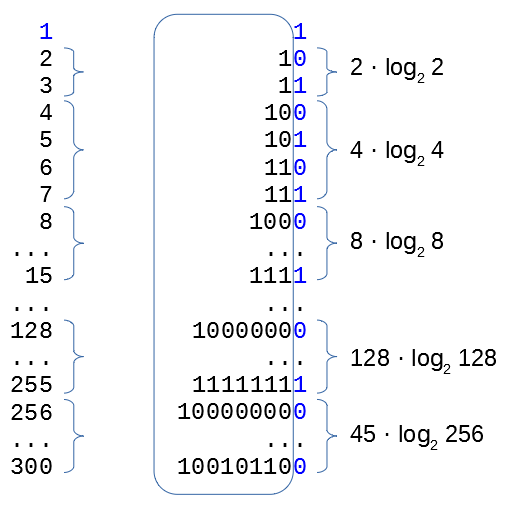
\includegraphics[width=2in]{online-competition-2021-04-08/q2-binary.png}}
\caption{\label{fig:q2-binary} Skaitļu no $1$ līdz $300$ binārie pieraksti.}
\end{figure}
}
\end{problem}


%%%%%%%%%%%%%%%
%%% 03 %%%%%%%%
%%%%%%%%%%%%%%%
\vspace{10pt}
\begin{problem}
Cik daudzi no pirmajiem $100$ naturālajiem skaitļiem $(1,\ldots,100)$ ir izsakāmi 
ar izteiksmi: 
\[ \lfloor 2x \rfloor + \lfloor 4x \rfloor + \lfloor 6x \rfloor + \lfloor 8x \rfloor. \]
Šeit $x$ var būt jebkurš reāls skaitlis.

{\bf Jautājums:} Ierakstīt skaitļu skaitu.
\answer{

{\bf Atbilde.} $\mathtt{60}$\\

Apzīmējam izteiksmi ar funkciju $f:\R \rightarrow \R$ (funkcija ar reāliem argumentiem un reālām vērtībām). 
Ja reālais mainīgais $x$ nepārtraukti palielinās no vērtības $x =0$ līdz vērtībai $x=5$, 
tad $f(x)$ vērtība pieaug no $f(0) = 0$ līdz $f(5)$ jeb
\[ \lfloor 2\cdot 5 \rfloor + \ldots + \lfloor 8 \cdot 5 = 10 + 20 + 30 + 40 = 100. \]

Ja aizstāj $x$ ar $x+0.5$, tad visi saskaitāmie $f(x)$ pieaug attiecīgi par $1,2,3,4$ (to veselo daļu summa pieaug 
par $1+2+3+4 = 10$) un tāpēc 
$f(x+0.5) = f(x) + 10$. Funkcijas $f(x)$ grafiks nav periodisks (jo vērtības pēc perioda neatgriežas agrākajās vietās), 
bet šis grafiks ir {\em simetrisks} pret paralēlajām pārnesēm par vektoru $(0.5,10)$. Tāpēc pietiek izpētīt, cik daudzas
vērtības $f(x)$ pieņem pusatvērtā intervālā $(0;0.5]$ (un paļauties uz to, ka tās vēlāk atkārtosies. Sk. Attēlu~\ref{fig:q3-staircase}.

\begin{figure}[!htb]
\center{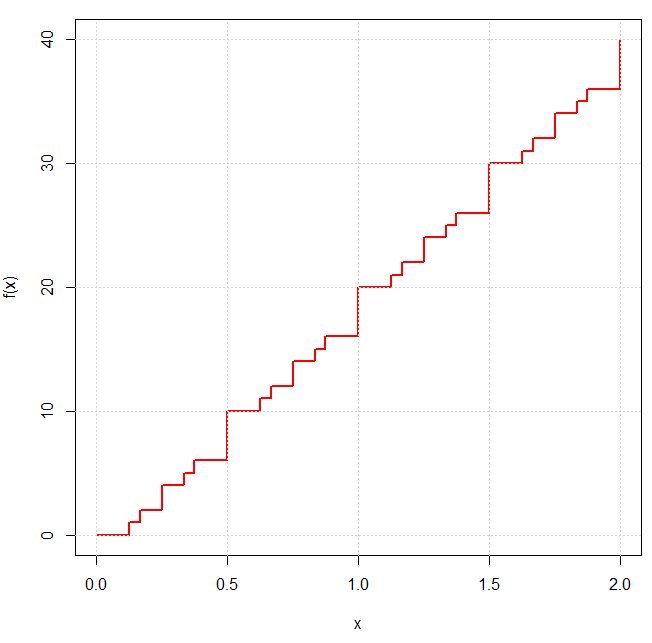
\includegraphics[width=3in]{online-competition-2021-04-08/q3-staircase.png}}
\caption{\label{fig:q3-staircase} Funkcijas $f(x) = \lfloor 2x \rfloor + \ldots + \lfloor 8x \rfloor$ grafiks.}
\end{figure}

Iegūstam šādas vērtības dažādiem $x \in (0;0.5]$:
\[ \left\{ \begin{array}{l}
f\left( \frac{1}{8} \right) = 1\\[2pt]
f\left( \frac{1}{6} \right) = 2\\[2pt]
f\left( \frac{1}{4} \right) = 4\\[2pt]
f\left( \frac{2}{6} \right) = 5\\[2pt]
f\left( \frac{3}{8} \right) = 6\\[2pt]
f\left( \frac{1}{2} \right) = 10\\
\end{array} \right. \]

Lai pārliecinātos, ka citu vērtību nav, varam vai nu rīkoties ar pilno pārlasi: aplūkot visus $12$ skaitļus
formā $\frac{k}{24}$, kur $k=1,2,\ldots,12$ (saucējs $24$ ir skaitļu $2,4,6,8$ mazākais kopīgais dalāmais; tātad
tikai šādām vērtībām $k/24$ ir iespējams, ka $2x$, $4x$, $6x$ vai $8x$ sasniedz veselu vērtību (un tātad mainās
izteiksmes $f(x)$ vērtība. 

Varam arī ievērot, ka pie $x = 1/4$ funkcija $f(x)$ ``palecas'' par divām vienībām (nav iespējama vērtība $f(x) = 3$, jo 
tai pārlec pāri). Savukārt pie $x = 1/2$ funkcija $f(x)$ ``palecas'' par četrām vienībām (nav iespējamas vērtības $7,8,9$). 
Atlikušās $6$ vērtības no kopas $\{1,2,3,5,6,10\}$ ir iespējamas pie $x \in (0;0.5]$. 

Pie $x$, kas pieder nākamajiem intervāliem $(0.5;1]$, vai $(1;1.5]$ utt. šis pats ritms atkārtojas. $f(x)$ grafika simetriskās
pārbīdes nodrošina, ka 
katrā nogrieznī $[1;10]$, $[11;20]$, utt. no $10$ veselajām vērtībām var dabūt tieši $6$. Tātad no garākā nogriežņa $[1;100]$
var dabūt $60$ vērtības.
%{\em Piezīme.} Grafika zīmēšanai piedāvājam R kodu: 
%\begin{Verbatim}
%f <- function(x) {
%  return (floor(2*x) + floor(4*x) + floor(6*x) + floor(8*x))
%}
%
%x <- seq(0.0, 2.0, by=0.001)
%plot(x,f(x),type='l', col="red", lwd=2)
%grid()
%\end{Verbatim}
}
\end{problem}


%%%%%%%%%%%%%%%
%%% 04 %%%%%%%%
%%%%%%%%%%%%%%%
\vspace{10pt}
\begin{problem}
Dots pozitīvs skaitlis $a$, kam $\{ a^{−1} \} =\{ a^2 \}$ un $2<a^2<3$. 
Atrast izteiksmes $a^{12}- 144 a^{-1}$ vērtību.

{\bf Jautājums:} Ierakstīt izteiksmes vērtību kā naturālu skaitli $\mathtt{N}$ vai racionālu daļu $\mathtt{P/Q}$.
\answer{

{\bf Atbilde.} $\mathtt{233}$\\

Tā kā $a^2 \in (2;3)$, var secināt arī, ka $a \in (1;2)$ un $a^{-1} \in (0;1)$.\\
Tāpēc daļveida daļa $\{ a^{-1} \} = a^{-1}$ (sakrīt ar pašu skaitli), bet $\{ a^2 \} = a^2 - 2$. 

Pārrakstām vienādojumu $\{ a^{−1} \} =\{ a^2 \}$; tad pareizinām abas puses ar $a$ un pārveidojam par kubisku vienādojumu:
\[ a^{−1} = a^2 - 2. \]
\[ 1 = a^3 - 2a. \]
\[ a^3 - 2a - 1 = 0. \]
Pēdējā vienādojuma risināšanai varam izmantot to, ka vienu sakni ($a = -1$) var uzminēt. 
Tāpēc polinomu $a^3 - 2a - 1$ var izdalīt ar $(a - (-1)) = a+1$. 

Var pārbaudīt šādu algebrisku identitāti: 
\[ a^3 - 2a - 1 = (a+1)(a^2 -a -1). \]
(Var vai nu atvērt iekavas, vai arī dalīt polinomus vienu ar otru.)

Sakne $a = -1$ neapmierina uzdevuma nosacījumus, tāpēc jārisina kvadrātvienādojums $a^2 - a - 1 = 0$. 
\[ a_{1,2} = \frac{1 \pm \sqrt{5}}{2}. \]
Vienīgā sakne, kas apmierina nosacījumus ir $a = \frac{1 + \sqrt{5}}{2} \approx 1.618034$. 
Tad $a^2 \approx 2.618034$, bet $a^{-1} \approx 0.618034$.

Aprēķinām izteiksmi $a^{12}-144 a^{-1}$:
\[ \left( \frac{1 + \sqrt{5}}{2} \right)^{12} - \frac{144}{\frac{1 + \sqrt{5}}{2}} = \]
\[ = \left(\left( \frac{1 + \sqrt{5}}{2}\right)^2 \right)^{6} - \frac{288}{1 + \sqrt{5}} = \]
\[ = \left(\frac{6 + 2\sqrt{5}}{4} \right)^6 - \frac{288(1 - \sqrt{5})}{(1 + \sqrt{5})(1 - \sqrt{5})} = \]
\[ = \left(\frac{3 + \sqrt{5}}{2} \right)^6 - \frac{288(1 - \sqrt{5})}{1 - 5} = \]
\[ = \frac{ 3^6 + C_6^1 3^5 \sqrt{5} + C_6^2 3^4 (\sqrt{5})^2 + C_6^3 3^3 (\sqrt{5})^3 + C_6^4 3^2 (\sqrt{5})^4 + C_6^5 3 (\sqrt{5})^5 + (\sqrt{5})^6}{64} + 72 (1 - \sqrt{5}) = \]
\[ = \frac{ 3^6 + 6 \cdot 3^5 \sqrt{5} + 15 \cdot 3^4 (\sqrt{5})^2 + 20 \cdot 3^3 (\sqrt{5})^3 + 15 \cdot 3^2 (\sqrt{5})^4 + 6  \cdot 3 (\sqrt{5})^5 + (\sqrt{5})^6}{64} + 72 (1 - \sqrt{5}) = \]
\[ = \frac{ 729 + 1458 \sqrt{5} + 1215 (\sqrt{5})^2 + 540 (\sqrt{5})^3 + 135 (\sqrt{5})^4 + 18 (\sqrt{5})^5 + (\sqrt{5})}{64} + 72 (1 - \sqrt{5}) = \]
\[ = \frac{ 729 + 1458 \sqrt{5} + 6075 + 2700 \sqrt{5} + 3375 + 450 \sqrt{5} + 125}{64} + 72 (1 - \sqrt{5}) = \]
\[ = \frac{ (729 + 6075 + 3375 + 125) + (1458 + 2700 + 450)\sqrt{5}}{64} + 72(1 - \sqrt{5}) = \]
\[ = 161 + 72 \sqrt{5} + 72(1 - \sqrt{5}) = 161 + 72\sqrt{5} + 72(1 - \sqrt{5}) = \]
\[ = (161 + 72) + (72 \sqrt{5} - 72 \sqrt{5}) = 233. \]

{\em Piezīme.} Ievērosim, ka $233$ ir Fibonači virknes loceklis: $F_{13} = 233$. Fibonači virknes
locekļus var aprēķināt ar izteiksmi, kurā arī ietilpst $\sqrt{5}$, tāpēc šāds iznākums nav sagadīšanās. 
Sk. \url{https://bit.ly/3sSq9Cw}.
}
\end{problem}



%%%%%%%%%%%%%%%
%%% 05 %%%%%%%%
%%%%%%%%%%%%%%%
\vspace{10pt}
\begin{problem}
Atrast mazāko naturālo skaitli $k$, pie kura vienādojumam 
\[ \left\lfloor \frac{2021}{n} \right\rfloor  = k \]
nav atrisinājuma veselos skaitļos.


{\bf Jautājums:} Ierakstīt atbildē naturālu skaitli $k$ ar šo īpašību.
\answer{

{\bf Atbilde.} $\mathtt{46}$\\

Virkne $a_n = \frac{2021}{n}$ ir dilstoša; turklāt tā dilst arvien lēnāk (un lieliem $n$ tuvojas vērtībai $0$). 
Pieņemsim, ka $n$ ir lielākā no tām $n$ vērtībām, kurai $\lfloor a_n \rfloor - \lfloor a_{n+1} \rfloor \geq 2$ (veselās 
daļas atšķiras vismaz par $2$. Jeb 
Lai vērtības $\lfloor 2021/n \rfloor$ ``pārlēktu'' pāri kādam veselam skaitlim, ir nepieciešams, lai 
divas pēc kārtas sekojošas virknes $a_n$ vērtības atšķirtos vairāk nekā par $1$ (jo citādi arī to veselās daļas
atšķirsies ne vairāk kā par $1$ vai neatšķirsies nemaz).

Uzrakstām šo 
kā nevienādību, kas jāizpilda mainīgajam $n$:
\[ \frac{2021}{n} - \frac{2021}{n+1} > 1. \]
Pārveidojam to par kvadrātisku nevienādību:
\[ 2021 \left( \frac{1}{n} - \frac{1}{n+1} \right) = 2021 \cdot \frac{1}{n(n+1)} > 1, \]
\[ 2021 > n^2 + n, \]
\[ n^2 + n - 2021 < 0. \]
Šim kvadrātvienādojumam ir viena pozitīva un viena negatīva sakne. Tā kā $n$ ir naturāls, tad tam jābūt mazākam 
par pozitīvo sakni: 
\[ n < \frac{-1 + \sqrt{1 + 4 \cdot 2021}}{2} = \frac{-1 + \sqrt{8085}}{2} \approx 44.45831. \]
Tāpēc lielākā $n$ vērtība, kurai $\lfloor a_n \rfloor - \lfloor a_{n+1} \rfloor \geq 2$ būs $n \leq 44$.

Ievietojam $2021/n$ vērtības $43$, $44$, $45$, $46$, $47$:
\[ \left\{ \begin{array}{l}
\frac{2021}{43} = 47.00000\\[2pt]
\frac{2021}{44} = 45.93182\\[2pt]
\frac{2021}{45} = 44.91111\\[2pt]
\frac{2021}{46} = 43.93478\\[2pt]
\frac{2021}{47} = 43.00000\\
\end{array} \right. \]
Iegūstam, ka pie $k = 46$ vienādojumam ${\displaystyle \left\lfloor \frac{2021}{n} \right\rfloor  = k}$ nav 
atrisinājuma veselos skaitļos. Savukārt visas $k$ vērtības, kuras ir vēl mazākas, tiks sasniegtas, jo dalījumi 
$2021/n$ (pie $n \geq 45$) samazinās par lielumiem, kas jau mazāki nekā $1$, t.i.\ šo lielumu veselās daļas
neizlaidīs vairs nevienu $k$ vērtību.
}
\end{problem}




%%%%%%%%%%%%%%%
%%% 06 %%%%%%%%
%%%%%%%%%%%%%%%
\vspace{10pt}
\begin{problem}
Dots, ka $\log_6 a + \log_6 b + \log_6 c= 6$, kur naturāli skaitļi $a,b,c$ veido augošu ģeometrisku progresiju un $b-a$ ir vesela skaitļa kvadrāts. Atrast $a,b,c$.


{\bf Jautājums:} Ierakstīt atbildē $a+b+c$ vērtību.
\answer{

{\bf Atbilde.} $\mathtt{111}$

Ja ģeometriskās progresijas kvocients ir $q$, tad $b = aq$ un $c = aq^2$. Ievietojam šīs vērtības logaritmu summā:
\[ \log_6 a + \log_6 b + \log_6 c = \log_6 a + \log_6 aq + \log_6 aq^2 = \log_6 a^3q^3 = 3 \log_6 aq = 6. \]
Tāpēc $\log_6 aq = 2$ jeb $\log_6 b = 2$. Iegūstam, ka vidējais ģeometriskās progresijas loceklis $b = 6^2 = 36$. 

Sadalām $36$ pirmreizinātājos: $36 = 2^2 \cdot 3^2$. Tāpēc arī skaitlim $a$ jāsatur tie paši pirmreizinātāji $2$ un $3$. 
(Ja skaitlī $a$ būtu vēl cits pirmreizinātājs $p \neq 2$ un $p \neq 3$, tad $c$ vairs nebūtu vesels, jo saturētu pirmskaitli 
$p$ saucējā un nebūtu ar ko to noīsināt.)

Vienīgie skaitļi ar pirmreizinātājiem $2$ un $3$, kuri nepārsniedz $b$ ir sekojoši: 
\[ 1,2,3,4,6,8,9,12,16,18,24,27,32. \]
Tie arī ir vienīgie skaitļa $a$ kandidāti (jo progresija $a,b,c$ ir augoša). 
Vienīgās $a$ vērtības no šī saraksta, kurām $b - a = 36 - a$ ir pilns kvadrāts ir $a_1 = 27$ un $a_2 = 32$. 

Vērtība $32$ neder, jo tad $c = b \cdot (b/a) = 36 \cdot (36/32) = 40.5$ nav naturāls.\\
Vērtība $27$ der, jo $c = b \cdot (b/a) = 36 \cdot (36 / 27) = 48$. 

Aprēķinām atbildi: $a+b+c = 27 + 36 + 48 = 111$.
}
\end{problem}



\begin{figure}[!htb]
\center{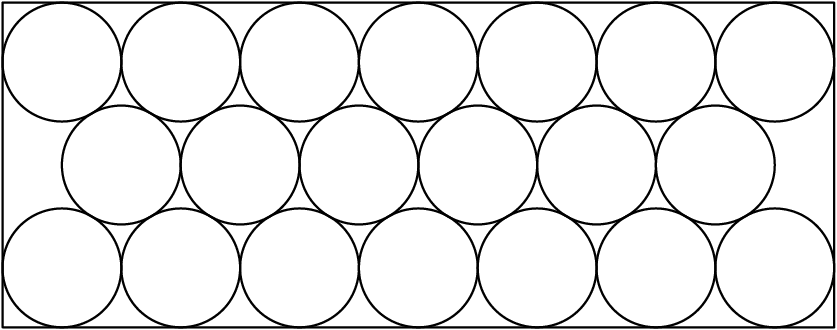
\includegraphics[width=2in]{online-competition-2021-04-08/q07-circles.png}}
\caption{\label{fig:q07-circles} Aplīši ievilkti taisnstūrī.}
\end{figure}

%%%%%%%%%%%%%%%
%%% 07 %%%%%%%%
%%%%%%%%%%%%%%%
\vspace{10pt}
\begin{problem}
Attēlā~\ref{fig:q07-circles} redzami $20$ kongruenti aplīši trīs rindās, kuriem no ārpuses pieskaras taisnstūris. 
Taisnstūra garākās malas attiecība pret īsāko ir uzdota ar formulu 
${\displaystyle \frac{\sqrt{a} - b}{2}}$, 
kur $a,b$ ir naturāli skaitļi. 
Atrast skaitļus $a,b$.



{\bf Jautājums:} Ierakstīt abus skaitļus $a,b$ (divi naturāli skaitļi, kurus atdala komats).
\answer{

{\bf Atbilde.} $\mathtt{147,7}$

Apzīmēsim viena aplīša rādiusu ar $r$ un izteiksim tiem apvilktā taisnstūra garāko malu $a$ un īsāko malu $b$. 
Attēlā~\ref{fig:q07-circles-equilateral} redzams, ka $a = 14r$. Savukārt īsākā mala $b = 4r \cdot \frac{\sqrt{3}}{2} + 2r$, jo 
tā vienāda ar vienu augstumu, kas novilkts vienādmalu trijstūrī ar malas garumu $2r$ (sarkanā krāsā) 
un vēl arī diviem rādiusiem (zilā krāsā). 
Iegūstam šādu garākās un īsākās malas attiecību: 
\[ \frac{14r}{4r \cdot \frac{\sqrt{3}}{2} + 2r} = \frac{7}{\sqrt{3} + 1} = \frac{7(\sqrt{3} - 1)}{(\sqrt{3} + 1)(\sqrt{3} - 1)} = \frac{\sqrt{147} - 7}{2}.\]


\begin{figure}[!htb]
\center{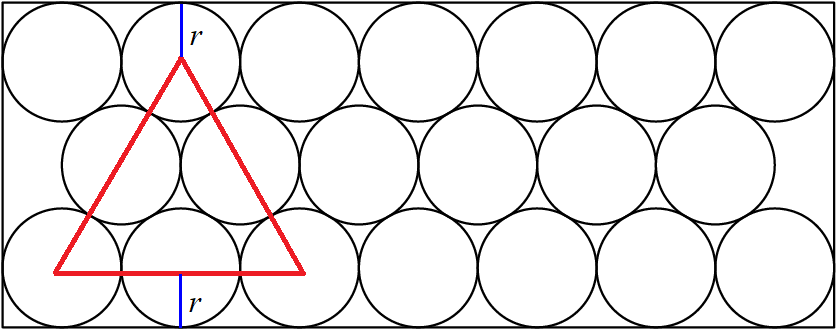
\includegraphics[width=3in]{online-competition-2021-04-08/q07-circles-equilateral.png}}
\caption{\label{fig:q07-circles-equilateral} Aplīši ievilkti taisnstūrī.}
\end{figure}
}
\end{problem}



%%%%%%%%%%%%%%%
%%% 08 %%%%%%%%
%%%%%%%%%%%%%%%
\vspace{10pt}
\begin{problem}
Uzrakstīt dotās izteiksmes vērtību kā racionālu skaitli $p/q$:
\[ \frac{2}{\log_4 2000^6} + \frac{3}{\log_5 2000^6}. \]

{\bf Jautājums:} Ierakstīt racionālu daļu $\mathtt{P/Q}$.
\answer{

{\bf Atbilde.} $\mathtt{1/6}$

Pārrakstām doto izteiksmi $E$, izmantojot dažas logaritmu īpašības (kāpinātāju var iznest pirms 
logaritma, $\log_a b = 1/(\log_b a)$ u.c.). 

\begin{align}
E = & \frac{2}{\log_4 2000^6} + \frac{3}{\log_5 2000^6} = \nonumber \\
 = & \frac{2}{6 \log_4 2000} + \frac{3}{6 \log_5 2000} = \nonumber \\
 = & \frac{1}{3} \cdot \frac{1}{\log_4 2000} + \frac{1}{2}\cdot \frac{1}{\log_5 2000} = \nonumber \\
 = & \frac{1}{3}\log_{2000} 4 + \frac{1}{2}\log_{2000} 5 = \nonumber \\
 = & \frac{1}{6}\left( 2 \log_{2000} 4 + 3 \log_{2000} 5 \right) = \nonumber \\
 = & \frac{1}{6}\left( \log_{2000} 4^2 + \log_{2000} 5^3 \right) = \nonumber \\
 = & \frac{1}{6} \log_{2000} \left( 4^2 \cdot 5^3 \right)  = \nonumber \\
 = & \frac{1}{6} \log_{2000} 2000  = \frac{1}{6}.\nonumber 
\end{align} 
}
\end{problem}



%%%%%%%%%%%%%%%
%%% 09 %%%%%%%%
%%%%%%%%%%%%%%%
\vspace{10pt}
\begin{problem}
Virknē
\[ 1000, x, 1000-x, \ldots \]
pirmie divi locekļi ir $a_0 = 1000$ un $a_1 = x$, bet katru nākamo $a_n$ iegūst atņemot iepriekšējo no tam iepriekšējā: $a_n=a_{n-2}- a_{n-1}$.
Virknes pēdējais loceklis ir pirmais negatīvais skaitlis, kas parādās šajā procesā. Kura naturāla $x$ vērtība rada visgarāko virkni?

{\bf Jautājums:} Ierakstīt veselu nenegatīvu skaitli \textendash{} to $x$ vērtību, kas dod visgarāko virkni.
\answer{

{\bf Atbilde.} $\mathtt{618}$\\

Ieviešam jaunu virkni $b_n = a_n/1000$, kur dalām visus virknes locekļus ar $1000$. 
\[ 1, x/1000, 1-x/1000, \ldots \]
Virknē $b_n$ pirmie locekļi ir $b_0 = 1$, $b_1 = t$, bet tālākie 
apmierina līdzīgu sakarību kā iepriekš: $b_n=b_{n-2}- b_{n-1}$, jo visas starpības un visi locekļi ir $1000$ reizes mazāki nekā virknē $a_n$.

Apzīmēsim $x/1000$ ar jaunu mainīgo $t$ (mums zināms, ka $t$ ir skaitlis, kura decimālpierakstā ir tieši trīs cipari aiz komata)
un izrakstīsim pirmos virknes $b_n$ locekļus (katru nākamo iegūst, izmantojot rekurenci $b_n=b_{n-2}- b_{n-1}$):
\begin{equation}
\label{eq:fibonacci-differences}
1,\; t,\; 1-t,\; 2t-1,\; 2-3t,\; 5t-3,\; 5-8t,\; 13t-8,\; 13-21t,\; 34t-21,\;  \ldots
\end{equation}
Apzīmēsim Fibonači skaitļu virkni (to definē šādi: $F_0 = 0$, $F_1 = 1$, $F_k=F_{k-1}+F_{k-2}$): 
\[ F_0=0,\; F_1=1,\; F_2=1,\; F_3=2,\; F_4=3,\; F_5=5,\; \ldots \]
Risinām vairākas nevienādību sistēmas mainīgajam $t$, lai nodrošinātu, ka iespējami daudzi virknes (\ref{eq:fibonacci-differences}) 
locekļi ir nenegatīvi:
\[ 
\left\{ \begin{array}{l}
t \geq 0 \\
1 - t \geq 0 \\
\end{array} \right.
\;\;\rightarrow\;\;
\left\{ \begin{array}{l}
t \geq 0 \\
t \leq 1 \\
\end{array} \right.\;\;
\;\;\rightarrow\;\;
t \in [0;1] \]
\[ 
\left\{ \begin{array}{l}
2t-1 \geq 0 \\
2-3t \geq 0 \\
\end{array} \right.
\;\;\rightarrow\;\;
\left\{ \begin{array}{l}
t \geq 1/2 \\
t \leq 3/2 \\
\end{array} \right.\;\;
\;\;\rightarrow\;\;
t \in \left[ \frac{1}{2};\frac{2}{3} \right] \]
\[ \left\{ \begin{array}{l}
5t-3 \geq 0 \\
5-8t \geq 0 \\
\end{array} \right.
\;\;\rightarrow\;\;
\left\{ \begin{array}{l}
t \geq 3/5 \\
t \leq 5/8 \\
\end{array} \right.\;\;
\;\;\rightarrow\;\;
t \in \left[ \frac{3}{5};\frac{5}{8} \right] \]
\[ \left\{ \begin{array}{l}
F_{2n+1}t-F_{2n} \geq 0 \\
F_{2n+1}-F_{2n+2}t \geq 0 \\
\end{array} \right.
\;\;\rightarrow\;\;
\left\{ \begin{array}{l}
t \geq F_{2n}/F_{2n+1} \\
t \leq F_{2n+1}/F_{2n+2} \\
\end{array} \right.\;\;
\;\;\rightarrow\;\;
t \in \left[ \frac{F_{2n}}{F_{2n+1}};\frac{F_{2n+1}}{F_{2n+2}} \right] \]
Izrakstām tabulā šo intervālu galapunktus, kuriem pieder skaitlis $t$ (līdzkamēr atrodam pirmo pretrunu). 

\begin{tabular}{|r||r|r|r|c|} \hline
$n$ & $F_{2n}$ & $F_{2n+1}$ & $F_{2n+2}$ & $[ F_{2n}/F_{2n+1}; F_{2n+1}/F_{2n+2}]$ \\ \hline
$0$ & $0$ & $1$ & $1$ & $[0.000000;1.000000]$ \\ \hline
$1$ & $1$ & $2$ & $3$ & $[0.500000;0.666667]$ \\ \hline
$2$ & $3$ & $5$ & $8$ & $[0.600000;0.625000]$ \\ \hline
$3$ & $8$ & $13$ & $21$ & $[0.615385;0.619048]$ \\ \hline
$4$ & $21$ & $34$ & $55$ & $[0.617647;0.618182]$ \\ \hline
$5$ & $55$ & $89$ & $144$ & $[0.617978;0.618056]$ \\ \hline
$6$ & $144$ & $233$ & $377$ & $[0.618026;0.618037]$ \\ \hline
\end{tabular}

Starp tām $t$ vērtībām, kas izsakāmas kā $x/1000$ veselam $x$ (decimālpierakstā tieši $3$ cipari aiz komata)
vislielākajam skaitam intervālu pieder skaitlis $t = 0.618$. Pirmā nevienādība, kura {\bf neizpildās}, 
ir $t \geq 0.618026 = F_{12}/F_{13}$. Tāpēc neizpildās arī $F_{13}t - F_{12} \geq 0$; tātad virknē $b_n$ (un arī $a_n$) 
pirmie $13$ locekļi (no nulltā līdz divpadsmitajam) ir nenegatīvi, bet jau četrpadsmitais loceklis $b_{13}$ (un arī $a_{13} = 1000 \cdot b_{13}$) 
ir negatīvs. 

Ievietojot $x = 618$ iegūstam šādu virkni: 
\[ 1000, 618, 382, 236, 146, 90, 56, 34, 22, 12, 10, 2, 8, -6. \]
}
\end{problem}


%%%%%%%%%%%%%%%
%%% 10 %%%%%%%%
%%%%%%%%%%%%%%%
\vspace{10pt}
\begin{problem}
Reāls skaitlis $r$ apmierina attēlā doto vienādību.
\[ \left\lfloor r+\frac{19}{100} \right\rfloor + \left\lfloor r+\frac{20}{100} \right\rfloor + 
\left\lfloor r+\frac{19}{100} \right\rfloor + \ldots + \left\lfloor r+\frac{91}{100} \right\rfloor = 546. \]

Atrast $\lfloor 100r \rfloor$. 

{\bf Jautājums:} Ierakstīt $\lfloor 100r \rfloor$ vērtību.
\answer{

{\bf Atbilde.} $\mathtt{743}$\\

%Ja pieņemam, ka $r = k/100$ (decimāldaļskaitlis ar tieši diviem cipariem aiz komata), tad vienādojums 
Izteiksmē ir $91 - 19 + 1 = 73$ saskaitāmie, jebkuri divi no tiem atšķiras ne vairāk kā par $1$. 
Noskaidrosim, cik un kādus saskaitāmos izvēlēties, lai to summa būtu $546$. 
Dalot $546$ ar $73$ (ar atlikumu) iegūsim: 
\[ 546 = 7 \cdot 73 + 35. \]
Tādēļ $546$ var iegūt, saskaitot $38$ septiņniekus un $35$ astoņniekus. 

$19 + 38 = 57$ ir mazākais no daļu skaitītājiem $n$, kam ${\displaystyle \left\lfloor r+\frac{n}{100} \right\rfloor}$ vienāds ar $8$. 
Atrisinām vienādojumu: 
\[ r + \frac{57}{100} = 8. \]
Pieskaitot mazākas daļas nekā $57/100$, veselajai daļai būs jānoapaļojas uz leju \textendash{} uz vērtību $7$. 

Iegūstam $r = 8 - 0.57 = 7.43$. Tāpēc $100r = 743$. 

{\em Piezīme.} Kā $r$ vērtības der arī visi citi skaitļi intervālā $r \in [7.43; 7.44)$, jo tiem visas veselās daļas
noapaļosies precīzi tāpat. Bet lielākām $r$ vērtībām, pareizais skaits ar ``septiņniekiem'' un ``astoņniekiem'' $73$ saskaitāmo 
summā tiks izjaukts, tās neder. Tāpēc noteikti jāizpildās $\lfloor 100r \rfloor = 743$. 
}
\end{problem}


\begin{center}
\rule{4in}{.4pt}
\end{center}

\vspace{5pt}
{\em (Vēl divi uzdevumi par racionāliem/iracionāliem skaitļiem, kuru nebija sākotnējā testā.)}


%%%%%%%%%%%%%%%
%%% 11 %%%%%%%%
%%%%%%%%%%%%%%%
\vspace{10pt}
\begin{problem}
Atrast, cik ir sakārtotu naturālu skaitļu pāru $(a,b)$, kuriem 
\[ \log_a b + 6 \log_b a = 5, \]
un $a,b < 2021$. 

{\bf Jautājums:} Ierakstīt veselu nenegatīvu skaitli: atrisinājumu $(a,b)$ skaitu.
\answer{

{\bf Atbilde.} $\mathtt{54}$\\

Apzīmējam $\log_a b = t$. Ievērosim arī, ka 
\[ \log_b a = \frac{\log_2 a}{\log_2 b} = \left( \frac{\log_2 b}{\log_2 a} \right)^{-1} = (\log_a b)^{-1} = \frac{1}{t}. \]
Tātad, samainot logaritmā bāzi un logaritmējamo skaitli, rodas apgrieztais skaitlis ($t$ pārtop par $1/t$). 
Ievietojam vienādojumā un pārveidojam:
\[ t + \frac{6}{t} = 5. \]
\[ t^2 + 6 = 5t. \]
\[ t^2 - 5t + 6 = 0. \]
Tātad $t = 2$ vai $t = 3$. Iegūstam, ka $\log_a b$ ir vai nu $2$ vai $3$. Tāpēc $b = a^2$ vai $b = a^3$. 
Skaitlis $a = 1$ nevar būt logaritma bāze; tāpēc atliek saskaitīt, cik ir pilnu kvadrātu un pilnu kubu, kuri mazāki par $2021$. 
Pilnie kvadrāti iespējami pie $a = 2,\ldots,44$. Iegūstam atrisinājumus formā $(a,a^2)$
\[ (2;4),\; (3;9),\; (4;16),\; \ldots,\; (44;1936). \]
Pilnie kubi iespējami pie $a = 2,3,\ldots,12$. Iegūstam atrisinājumus formā  $(a,a^3)$
\[ (2;8),\; (3;27),\; (4;64),\; \ldots,\; (12; 1728). \]

Šo atrisinājumu pavisam ir $43 + 11 = 54$. 

{\em Piezīme.} Dažas $b$ vērtības (piemēram $2^6 = 64$ vai $3^6 = 729$) var būt gan pilni kvadrāti, gan pilni kubi; bet
tad tās piedalās divos dažādos atrisinājumos; piemēram $(a;b) = (8;64)$ un arī $(a;b) = (4;64)$. Un tās jāieskaita abas reizes, 
kā arī esam darījuši.
}
\end{problem}



%%%%%%%%%%%%%%%
%%% 12 %%%%%%%%
%%%%%%%%%%%%%%%
\vspace{10pt}
\begin{problem}

Atrast $(x+1)^{48}$, kur
\[ x = \frac{4}{(\sqrt{5}+1)(\sqrt[4]{5}+1)(\sqrt[8]{5}+1)(\sqrt[16]{5}+1)}. \]

{\bf Jautājums:} Ierakstīt vērtību kā naturālu skaitli $\mathtt{N}$ vai racionālu daļu $\mathtt{P/Q}$.
\answer{

{\bf Atbilde.} $\mathtt{125}$\\

Reizinām izteiksmes skaitītāju un saucēju ar $(\sqrt[16]{5}-1)$, lai vairākkārt izmantotu kvadrātu starpības formulu: 
\begin{align}
x = & \frac{4(\sqrt[16]{5}-1)}{(\sqrt{5}+1)(\sqrt[4]{5}+1)(\sqrt[8]{5}+1)(\sqrt[16]{5}+1)(\sqrt[16]{5}-1)} = \nonumber \\
 = &  \frac{4(\sqrt[16]{5}-1)}{(\sqrt{5}+1)(\sqrt[4]{5}+1)(\sqrt[8]{5}+1)(\sqrt[8]{5}-1)} = \nonumber \\
 = &  \frac{4(\sqrt[16]{5}-1)}{(\sqrt{5}+1)(\sqrt[4]{5}+1)(\sqrt[4]{5}-1)} = \nonumber \\
 = &  \frac{4(\sqrt[16]{5}-1)}{(\sqrt{5}+1)(\sqrt{5}-1)} = \nonumber \\
 = &  \frac{4(\sqrt[16]{5}-1)}{5-1} = \sqrt[16]{5}-1. \nonumber 
\end{align}

Tāpēc $x+1 = \sqrt[16]{5}$ un $(x+1)^{48} = 5^3 = 125$. 
}
\end{problem}


\end{document}









